% filepath: /Users/xiangjiahao/tex/weekly_report/2024/12/2024-12-23.tex
\documentclass[11pt,a4paper]{article}
\usepackage{ctex}
\usepackage[utf8]{inputenc}
\usepackage{geometry}
\usepackage{fancyhdr}
\usepackage{enumitem}
\usepackage{titlesec}
\usepackage{amsmath} % Added for math equation support
\usepackage{amssymb}
\usepackage{graphicx} % Added for including graphics
\usepackage{titling}
\usepackage{subcaption}
\usepackage{multicol}
\usepackage{listings}
\usepackage{booktabs}
\usepackage{multirow}
\usepackage[hidelinks]{hyperref}

\geometry{margin=0.5in}
\titleformat{\section}{\large\bfseries}{\thesection}{0.5em}{}
\title{周报-向嘉豪(2024-12-23)}
\setlength{\droptitle}{-6em}

\renewcommand{\maketitle}{
  \begin{center}
    \LARGE\bfseries\thetitle
  \end{center}
}

\begin{document}

\maketitle

\noindent \textbf{摘要}:围绕密码实现的关键需求与最新技术进展展开讨论,强调了安全性、性能与成本之间的平衡。在综合分析了硬件加速与软件实现的异同后,我们确定了以GPU为基础的异构加速策略。这一方案兼具较高的安全等级、合理的经济成本和出色的执行效率,尤其适用于对性能要求处于中等水平的应用场景。结果显示,软硬件结合能够在安全需求和可承受预算之间实现最佳折中,最终为进一步深入研究提供了明确方向。

\vspace{1em}
\noindent \textbf{下周计划}:完善针对GPU加速的技术研究,以深入量化并评估加密算法实现在异构环境中的表现。

\section{第二篇投稿}
对于第二篇投稿,我们在准备材料的过程中,深入研究了\textit{Computer}期刊对应的投稿要求与选题方向,并完成了针对最合适Topic的初步匹配。由于个人Biography信息不全导致稿件被退回,我们立即补充完成了该部分内容并再次提交,以期快速进入下一轮审查环节。

\section{第三篇论文背调}
在第三篇论文的背景调研中,我们着重考察了密码实现过程中的安全性、性能与成本三者间的关联(如图\ref{fig:tradeoff}所示),发现如果在相同安全等级下提升性能,成本便会随之增加;而在相同性能标准下提升安全性,同样会带来更高的成本。若成本固定且目标是保持较高的安全性并兼顾一定的性能要求,那么软硬件结合就能够在绿色和蓝色区域之外实现平衡,形成文中所述的红色区域范围。我们调研了多种硬件加速方案,包括FPGA实现与定制指令集,如《RISC-V instruction set extensions for lightweight symmetric cryptography》 CHES - 2023,和GPU作为异构加速平台,如《Efficient implementation of AES-CTR and AES-ECB on GPUs with applications for high-speed FrodoKEM and exhaustive key search》Trans on Circuits and Systems - 2022。考虑到实验环境的搭建环境和成本,我们最终选择了GPU作为异构加速平台,以实现对性能要求处于中等水平的应用场景。

\begin{figure}[h]
    \centering
    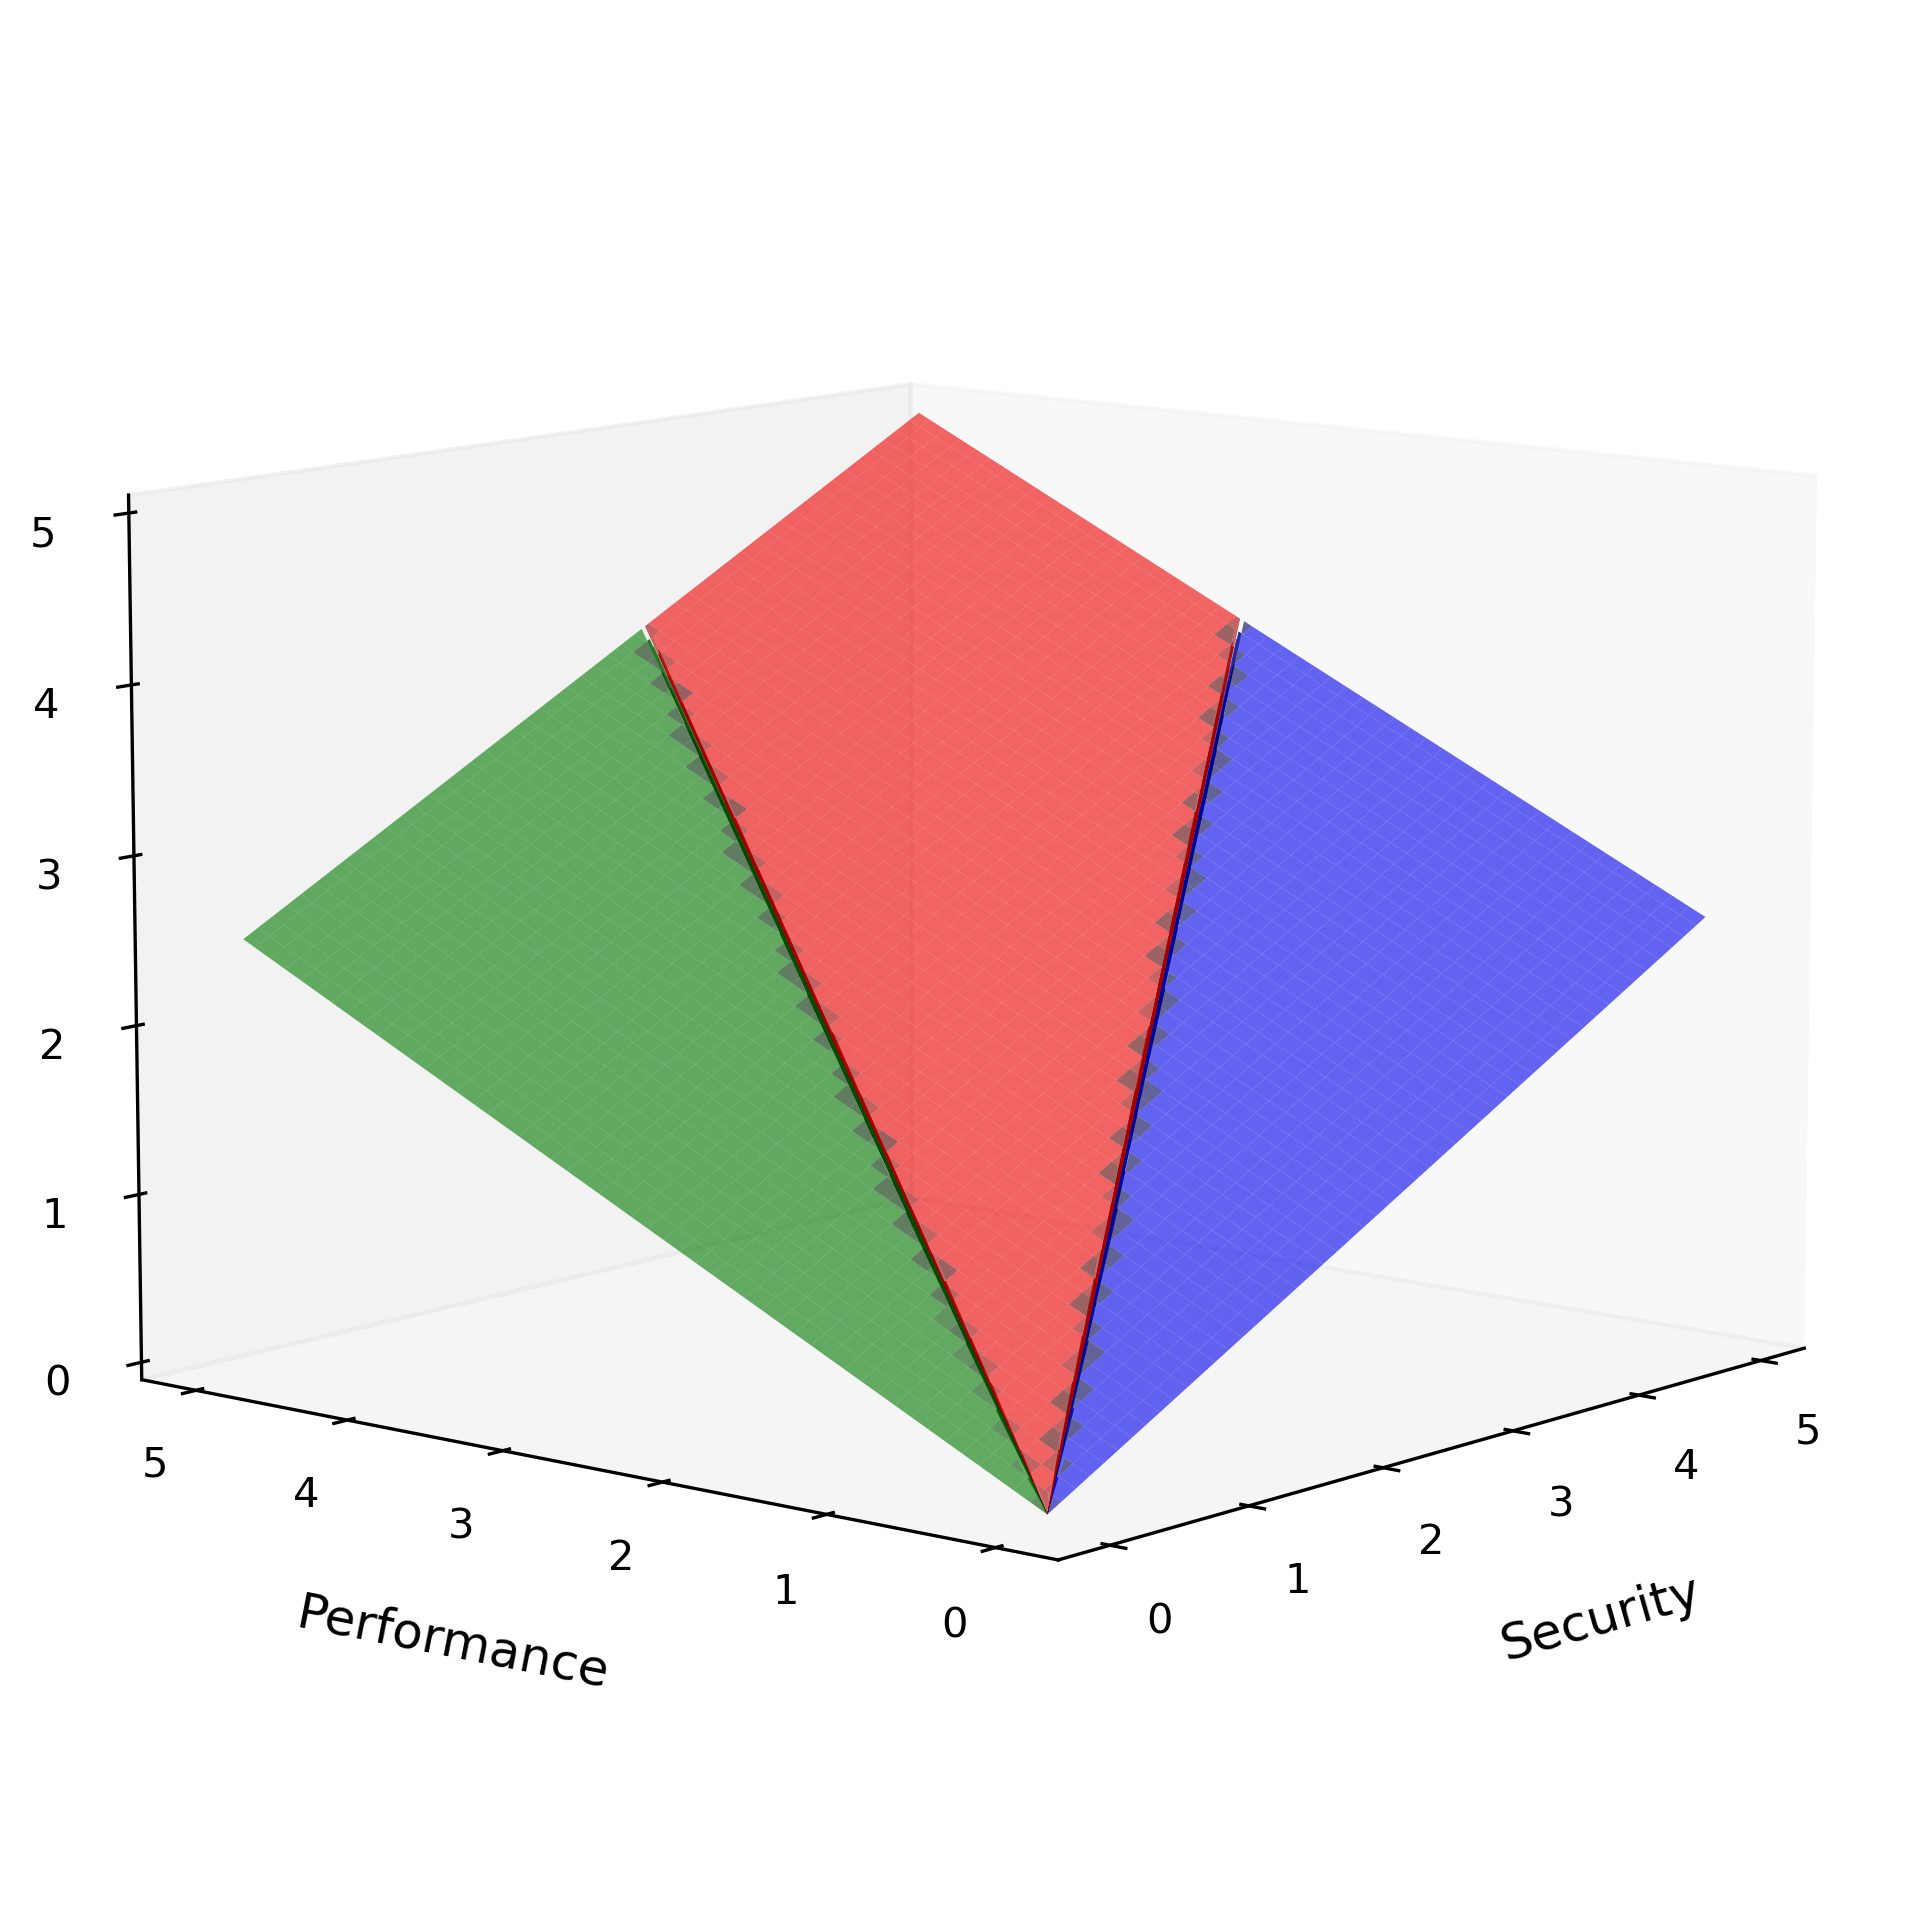
\includegraphics[width=0.45\textwidth]{./fig/SPC_relation.png}
    \caption{安全性、性能和成本间的关系}
    \label{fig:tradeoff}
\end{figure}

\end{document}